\RequirePackage{etex}
\documentclass[12pt,a4paper]{report}

% Packages de base
\usepackage[utf8]{inputenc}
\usepackage[T1]{fontenc}
\usepackage[french]{babel}
\usepackage{lmodern}
\usepackage{geometry}
\usepackage[french]{babel}
\usepackage{setspace}
\usepackage{float}
\usepackage{placeins}
\usepackage{enumitem}
\usepackage{graphicx}
\usepackage{amsmath, amssymb}
\usepackage{hyperref}
\usepackage{csquotes} 
\usepackage{tocbibind} % Pour inclure la bibliographie dans la table des matières
\usepackage{svg}
\usepackage{tabularx}
\usepackage{booktabs}
\usepackage{array}
\usepackage{caption}
\usepackage{subcaption}
\usepackage{pgfmath} 
\usepackage{etex} % Étend la capacité mémoire de LaTeX
\usepackage{pgfplotstable} %Pour les celules dynamyques dans un tableau
\usepackage{tabularray} % Pour tableau plus dynamyque
\pgfplotsset{compat=1.18}

\geometry{left=2.5cm, right=2.5cm, top=2.5cm, bottom=2.5cm}
\onehalfspacing

\usepackage{titlesec}

\titleformat{\chapter}[hang]
  {\normalfont\huge\bfseries} 
  {\thechapter.}              
  {1em}                      
  {\Huge}

\titlespacing*{\chapter}{0pt}{-20pt}{20pt}

\usepackage{etoolbox}
\makeatletter
\patchcmd{\@makechapterhead}{\vspace*{50\p@}}{\vspace*{0pt}}{}{}
\patchcmd{\@makeschapterhead}{\vspace*{50\p@}}{\vspace*{0pt}}{}{}
\makeatother

\geometry{left=2.5cm, right=2.5cm, top=2.5cm, bottom=2.5cm}
\onehalfspacing

\titleformat{\chapter}[display]
  {\normalfont\huge\bfseries}{}{0pt}{\Huge}

\titleformat{\chapter}[hang]
  {\normalfont\huge\bfseries} 
  {\thechapter.}              
  {1em}                      
  {\Huge}                    
\setlength{\parindent}{0pt}

\begin{document}

\begin{titlepage}
    \centering
    
\includegraphics[width=0.4\textwidth]{logoSorbonne.png}\par
    \vspace{1cm}
    
    {\scshape\LARGE Sorbonne Université \par}
    \vspace{1.5cm}
    
    {\scshape\Large Sciences du Langage\par}
    \vspace{0.5cm}
    
    {\scshape\Large Langue et Informatique\par}
    \vspace{1.5cm}
    
    {\huge\bfseries Annie Ernaux et l'écriture plate\par}

    \vspace{0.5cm}
    {\Large Une modélisation simple à partir d’analyses lexicales, syntaxiques et rhétoriques\par}
    \vspace{2cm}
    
    {\Large Présenté par : Ruixing ZHENG\par}
    \vspace{0.5cm}
    
    {\large Sous la direction de :  
    Gaël LEJEUNE\par}
    \vfill
    
    {\Large Soutenu le 15/05 2025\par}
\end{titlepage}






% Table des Matières
\tableofcontents
\newpage

%Introduction
\chapter{Introduction}
Depuis la publication de son premier roman \textit{Les Armoires vides} en 1974, la quête centrale d’Annie Ernaux est restée celle de l’expression authentique de toutes les dimensions de l’expérience vécue. Après la parution de trois romans de jeunesse (\textit{Les Armoires vides}, \textit{Ce qu’ils disent ou rien}, \textit{La Femme gelée}), Ernaux s’est tournée résolument vers une écriture mêlant autobiographie sociale, forme diaristique et observation extérieure. En 1984, elle obtient le prix Renaudot pour \textit{La Place}, et établit progressivement un style d’écriture fondé sur une langue épurée, directe et dénuée d’ornement, pour retranscrire la vie intime, la souffrance et la mémoire collective. Ce style, qui s’impose comme une des marques de la littérature française des années 1980, est aujourd’hui reconnu comme une forme singulière, qualifiée d’\textit{écriture plate}. Toutefois, sa définition précise dans le champ du traitement automatique du langage (TAL) reste encore largement inexplorée.\\

Cette étude vise donc à caractériser systématiquement, à l’aide de méthodes d’analyse quantitative, les traits linguistiques (lexicaux, syntaxiques et rhétoriques) propres à chaque œuvre d’Ernaux, afin de rendre compte de l’évolution stylistique de son écriture, depuis les expérimentations des débuts jusqu’à la maturité formelle de la période tardive. Par ailleurs, cette recherche pose la question suivante : l’\textit{écriture plate} est-elle une invention esthétique propre à Ernaux, ou bien reflète-t-elle une tendance stylistique partagée par les écrivains français de la seconde moitié du XX\textsuperscript{e} siècle ? \\

Nous organisons la suite de cette contribution de la façon suivante : dans la section 2, nous présentons brièvement une revue des travaux utilisant des outils numériques pour l’identification des caractéristiques stylistiques dans les œuvres littéraires ; la section 3 décrit notre corpus, notre méthodologie et les outils de visualisation numériques; les sections 4 et 5 exposent et analysent en détail les résultats de nos expérimentations ; enfin, la section 6 synthétise les conclusions de notre étude et propose des pistes pour de futures recherches.

%Etat de l'art
\chapter{Etat de l'art}
\label{chap:Etat_de_l'art}
L’analyse du style littéraire à l’aide d’outils numériques constitue aujourd’hui un champ de recherche dynamique au croisement de la linguistique computationnelle et des études littéraires. Les approches combinant méthodes quantitatives et interprétation stylistique ont permis d’éclairer de nouvelles dimensions formelles dans des œuvres appartenant à diverses époques et traditions. Dans cette section, nous présentons plusieurs travaux qui ont marqué ce domaine et dont les apports méthodologiques nourrissent notre propre démarche.\\

\par Le cadre théorique d’analyse du style littéraire dans les romans français du XIX\textsuperscript{e} siècle, élaboré par Lu Yuanfeng dans sa thèse de doctorat, démontre de manière convaincante la capacité des schémas syntaxiques à distinguer les styles littéraires. En combinant l’analyse syntaxique en dépendances avec la modélisation statistique via le système UDPipe, il construit un modèle quantitatif innovant permettant non seulement de valider mais aussi de remettre en question certaines conceptions traditionnelles sur le style des écrivains. Parallèlement, Garric et Maurel-Indart, dans leur ouvrage \textit{Vers une automatisation de l’analyse textuelle}, ancrent leur réflexion autour de la problématique interdisciplinaire suivante : dans quelle mesure un style peut-il être modélisé et reconnu automatiquement ? À travers une étude de cas portant sur \textit{La Princesse de Clèves}, ils explorent systématiquement les possibilités théoriques d’une telle analyse automatisée du style.\\

\par Ces recherches démontrent non seulement l’efficacité des approches syntaxiques et statistiques dans l’identification des styles, mais elles constituent également une base méthodologique solide pour la caractérisation de l’\textit{écriture plate} dans un cadre de traitement automatique des langues (TAL). En particulier, le travail de modélisation de Lu sur les styles narratifs du XIX\textsuperscript{e} siècle montre comment les structures syntaxiques peuvent révéler des différences systématiques entre les auteurs — un apport précieux pour la compréhension des traits de simplicité et de dépouillement caractéristiques de l’écriture d’Annie Ernaux. De plus, la question de la « modélisabilité » du style posée par Garric et Maurel-Indart résonne avec notre problématique centrale : dans quelle mesure un style d’écriture peut-il être formalisé, identifié par des moyens computationnels, et ainsi se voir attribuer une valeur esthétique distincte ?\\

\par Or, bien que de nombreuses études aient exploré les liens entre style, syntaxe, lexique ou figures rhétoriques, la modélisation systématique de l’\textit{écriture plate} en tant que genre stylistique spécifique demeure encore largement absente. Dans le contexte de la littérature française contemporaine, les recherches sur l’\textit{écriture plate} se concentrent principalement sur des analyses philosophiques ou narratives, sans proposer de description opérationnelle de ses caractéristiques linguistiques.\\

\par Dans ce contexte, notre étude postule qu’une analyse stylistique efficace doit articuler plusieurs dimensions : une mesure précise des indicateurs quantitatifs (TTR, longueur moyenne des phrases, diversité syntaxique, etc.), une validation croisée par des analyses qualitatives, ainsi qu’une mise en perspective comparative avec d’autres auteurs du même contexte littéraire. L’objectif est de déterminer si l’\textit{écriture plate} constitue un registre stylistique identifiable, susceptible d’être situé dans une généalogie esthétique cohérente.


%Méthodologie
\chapter{Méthodologie} \label{chap:Méthodologie}
\section{Le corpus d’étude}

Le corpus utilisé dans cette étude comprend deux ensembles. Le premier est un corpus interne constitué de l’ensemble des œuvres publiées par Annie Ernaux, couvrant une période allant de \textit{Les Armoires vides} (1974) à \textit{Le Jeune Homme} (2022). Afin d’observer l’évolution stylistique de son écriture, nous avons classé ces textes en différentes catégories génériques, notamment les romans de jeunesse, les journaux intimes ou extimes, et les récits que nous supposons appartenir à l’esthétique de l’\textit{écriture plate}. Cette catégorisation est fondée à la fois sur des critères éditoriaux, critiques et stylistiques. Le tableau \ref{table:corpus_interne} présente l’ensemble des œuvres d’Annie Ernaux et leur classification dans le corpus interne.|\\


Le second corpus est un corpus externe, composé de 15 œuvres de 9 auteurs qui représentent des courants littéraires importants de la littérature francophone de l'après-guerre jusqu'aux années 1970 : l'existentialisme (Camus, Sartre), le Nouveau Roman (Robbe-Grillet, Sarraute, Simon, etc.), ainsi que des auteurs à la profondeur historique et culturelle telle que Yourcenar. Parmi les auteurs masculins figurent Albert Camus, Jean-Paul Sartre, Michel Tournier, Alain Robbe-Grillet, Robert Pinget, et Claude Simon. Les auteures féminines incluent Nathalie Sarraute, Marguerite Yourcenar, et Moira. Leurs œuvres serviront de points de comparaison stylistique pour situer Ernaux dans le paysage littéraire de son époque.Le tableau \ref{table:corpus_externes} présente les titres des œuvres choisies pour le corpus externe, ainsi que les auteurs associés.




\begin{table}[h!]
\centering
\begin{tabular}{|l|l|l|}
\hline
\textbf{Titre}                       & \textbf{Année} & \textbf{Catégorie}     \\ \hline
Les Armoires vides                   & 1974           & De jeunesse            \\ \hline
Ce qu'ils disent ou rien             & 1977           & De jeunesse            \\ \hline
La Femme gelée                       & 1981           & De jeunesse            \\ \hline
La Place                             & 1983           & Plate ?                \\ \hline
Une Femme                            & 1987           & Plate ?                \\ \hline
Passion simple                       & 1991           & Plate ?                \\ \hline
Journal du dehors                    & 1993           & Journal extime         \\ \hline
Je ne suis pas sortie de ma nuit     & 1997           & Journal                \\ \hline
La Honte                             & 1997           & Plate ?                \\ \hline
L'événement                          & 2000           & Plate ?                \\ \hline
Se Perdre                            & 2001           & Plate ?                \\ \hline
L'Autre Fille                        & 2001           & Plate ?                \\ \hline
L'Occupation                         & 2002           & Plate ?                \\ \hline
Les Années                           & 2008           & Plate ?                \\ \hline
L'Atelier noir                       & 2011           & Journal                \\ \hline
Retour à Yvetot                      & 2013           & Plate ?                \\ \hline
Regarde les lumières mon amour       & 2014           & Journal extime         \\ \hline
Mémoire de fille                     & 2016           & Plate ?                \\ \hline
Le jeune homme                       & 2022           & Plate ?                \\ \hline
\end{tabular}
\caption{Corpus interne (œuvres d'Annie Ernaux)}
\label{table:corpus_interne}
\end{table}

\begin{table}[h!]
\centering
\begin{tabular}{|l|l|}
\hline
\textbf{Titre}                                        & \textbf{Auteur}     \\ \hline
C\_1951\_Camus\_Chute.txt                              & Camus               \\ \hline
C\_1964\_Sartre\_Mots.txt                              & Sartre              \\ \hline
C\_1967\_Tournier\_Vendredi.txt                        & Tournier            \\ \hline
C\_1975\_Tournier\_Meteores.txt                        & Tournier            \\ \hline
C\_1950-1972\_Green\_Moira.txt                         & Green               \\ \hline
L\_1959\_Sarraute\_Planetarium.txt                     & Sarraute            \\ \hline
L\_1967\_Simon\_Histoire.txt                           & Simon               \\ \hline
L\_1955\_RobbeGrillet\_Jalousie.txt                    & Robbe-Grillet       \\ \hline
L\_1962\_Pinget\_Inquisitoire.txt                      & Pinget              \\ \hline
L\_1976\_Sarraute\_Disent.txt                          & Sarraute            \\ \hline
yourcenar\_homme-obscur\_une-belle-matinee.txt         & Yourcenar           \\ \hline
yourcenar\_souvenirs-pieux.txt                         & Yourcenar           \\ \hline
yourcenar\_archives-du-nord.txt                        & Yourcenar           \\ \hline
yourcenar\_oeuvre-au-noir.txt                          & Yourcenar           \\ \hline
yourcenar\_memoires-hadrien.txt                        & Yourcenar           \\ \hline
\end{tabular}
\caption{Corpus externe (auteurs contemporains)}
\label{table:corpus_externes}
\end{table}

\clearpage

\section{Approche méthodologique}
Tout d'abord, nous procédons au traitement du corpus en affichant les données existantes et en les nettoyant afin d'assurer l'exactitude et la cohérence des données. Ensuite, nous entamons la phase de recherche proprement dite.\\

Premièrement, au niveau lexical, nous identifierons le thème de chaque œuvre afin de comprendre le contenu principal de chaque texte. Nous analyserons également les verbes et les auxiliaires utilisés dans chaque œuvre, en étudiant la répartition des temps verbaux, en particulier la variation des temps entre les œuvres de jeunesse et celles plus récentes. De plus, nous examinerons l'utilisation des pronoms dans chaque œuvre, en nous concentrant sur les pronoms de première personne ``je'', les pronoms de troisième personne ``elle'', ``il'', ``elles'', ``ils'', ainsi que les pronoms représentant des groupes ou des interactions, tels que ``nous'' et ``vous'', en étudiant leur fréquence d'apparition. Nous analyserons également la distribution de ces pronoms dans les œuvres plus anciennes et plus récentes. Par ailleurs, nous évaluerons le nombre moyen de mots et de caractères par œuvre, afin de mieux comprendre la structure des phrases dans chaque texte. Enfin, nous introduirons l'indice TTR (Type-Token Ratio), qui analyse le rapport entre le nombre de mots différents et le nombre total de mots, pour observer la richesse lexicale de chaque œuvre et comparer cette richesse entre les œuvres de jeunesse et les plus récentes.\\

Deuxièmement, au niveau de la structure syntaxique, nous procéderons à un marquage morphosyntaxique des tokens pour observer la proportion de différents types de mots, notamment les adverbes, les adjectifs, les conjonctions de coordination, les conjonctions subordonnées et les noms, et analyser les différences structurelles entre les œuvres de jeunesse et les plus récentes.\\

Troisièmement, au niveau des figures de style, nous nous concentrerons sur la densité des répétitions et des parallélismes dans chaque œuvre, en comparant leur fréquence d'utilisation dans les œuvres anciennes et récentes. Étant donné que d'autres figures de style, comme les métaphores et les comparaisons, sont plus difficiles à quantifier, notre étude se concentrera principalement sur ces deux figures.\\

Grâce à ces analyses, nous obtiendrons des résultats quantitatifs sur les trois dimensions : lexicale, syntaxique et stylistique pour chaque œuvre, et nous pourrons observer les différences entre les œuvres de jeunesse et les œuvres plus récentes. Cela nous permettra de répondre aux questions suivantes :
\begin{enumerate}
    \item Les œuvres d'Annie Ernaux présentent-elles réellement une caractéristique de ``binarité'' absolue ?
    \item Les différences entre ses œuvres de jeunesse et ses œuvres récentes sont-elles réellement significatives ?
    \item Peut-on identifier des éléments syntaxiques et stylistiques qui traversent l'ensemble de ses œuvres ?
    \item Devons-nous affiner, nuancer, ou au contraire confirmer la transformation esthétique qu'Annie Ernaux évoque à partir de sa quatrième œuvre, afin de redéfinir plus concrètement ce qu'elle entend par ``écriture plate'' ?
\end{enumerate}


Enfin, en nous appuyant sur la définition de l' ``écriture plate'' que nous aurons développée à partir de cette étude, nous analyserons les valeurs du TTR et les fréquences moyennes des œuvres du corpus externe, pour observer si nous pouvons y reconnaître des caractéristiques de ce style d'écriture , et déterminer si il est spécifique à Annie Ernaux.

\section{Outils de visualisation numérique utilisés}

Dans le cadre de cette étude, nous avons utilisé divers outils de visualisation afin de représenter graphiquement les données textuelles analysées. Ces outils facilitent la compréhension des tendances linguistiques, des caractéristiques de distribution et de leur évolution au sein des œuvres étudiées :\\


\textbf{Diagrammes en barres (bar plots)} : Ce type de graphique permet de comparer visuellement les fréquences ou les moyennes entre différentes catégories. Par exemple, nous avons utilisé des diagrammes en barres pour représenter la fréquence d’utilisation des pronoms, la répartition des temps verbaux, ainsi que la moyenne du nombre de mots par œuvre.\\

\textbf{Boîtes à moustaches (box plots)} : Les diagrammes en boîte offrent une représentation synthétique de la distribution d’un ensemble de données en indiquant la médiane, les quartiles et les éventuels points aberrants. Ils sont particulièrement adaptés pour comparer la variabilité de certains indicateurs linguistiques (comme la valeur du TTR ou la richesse lexicale) entre les œuvres de jeunesse et les œuvres plus récentes.\\

\textbf{Nuages de mots (word clouds)} : Les nuages de mots sont une forme de visualisation fondée sur la fréquence des mots, où la taille d’un mot est proportionnelle à sa fréquence d’apparition dans le texte. Ils permettent une première exploration qualitative des lexiques dominants dans chaque œuvre ou groupe d’œuvres, et peuvent révéler des thèmes récurrents ou des évolutions lexicales.\\

En complément, nous avons également utilisé le \textbf{TTR (Type-Token Ratio, ratio types-tokens)}, un indicateur important permettant de mesurer la richesse lexicale d’un texte, largement utilisé en linguistique. Le TTR se calcule en divisant le nombre de mots différents (\textit{types}) par le nombre total de mots (\textit{tokens}) dans un texte. Les \textit{types} désignent tous les mots distincts (chaque mot n’est compté qu’une seule fois), tandis que les \textit{tokens} incluent l’ensemble des mots, y compris les répétitions.\\

La valeur du TTR reflète la diversité lexicale d’un texte : un TTR élevé indique une plus grande diversité de vocabulaire, tandis qu’un TTR faible traduit une utilisation plus répétitive du lexique. Dans notre étude, nous avons utilisé le TTR pour comparer la richesse lexicale des différentes œuvres, en nous intéressant particulièrement aux différences entre les œuvres de jeunesse et les œuvres récentes d’Annie Ernaux. Cette analyse permet de mettre en lumière l’évolution stylistique de l’autrice : par exemple, une diminution du TTR pourrait indiquer une simplification du langage et un style plus direct, associé à l’esthétique d’une « écriture plate » ; à l’inverse, une augmentation du TTR pourrait signaler un enrichissement lexical et une complexité croissante du style.


%Résultats
\chapter{Résultats}
\label{chap:Résultats}
\input{04_Résultats}

%Analyse et discussion
\chapter{Analyse et discussion}
\label{chap:Analyse_et_discussion}
\section{Corpus interne}

\subsection{Analyse lexicale}
À travers l’analyse des nuages de mots des différentes œuvres d'Ernaux, on peut observer les différences et évolutions thématiques entre ses écrits, reflétant l’évolution de son contenu au fil du temps. Globalement, les premiers travaux se concentrent sur des mots-clés liés aux noms de personnes, aux lieux, à l’éducation et aux rôles sociaux, ce qui témoigne de l'expérience personnelle et du contexte familial de l’auteure. Les thèmes abordés sont centrés sur des personnages concrets et l’expérience de l’enfance. Les œuvres ultérieures, quant à elles, s'orientent davantage vers des mots-clés liés au corps, aux institutions, à la mémoire, à la politique et aux scènes sociales, manifestant une exploration approfondie des expériences féminines, de la mémoire collective et des mécanismes sociaux et culturels. Le vocabulaire met également en évidence un changement significatif : les premiers travaux se concentrent principalement sur des récits familiaux et de croissance centrés sur "moi - ma mère - l’école", tandis que les œuvres plus récentes se tournent vers des perspectives sociales et corporelles avec des explorations sur "le corps - le pouvoir - la mémoire".\\

Plus précisément, dans ses premiers écrits, comme \textit{Les Armoires vides}, des mots-clés tels que "denise", "école", "boutique", "épicerie" révèlent son expérience d’enfance, son origine sociale et son environnement de croissance. Dans \textit{La Femme gelée}, des termes comme "brigitte", "garçons", "bouffe", "liberté" indiquent une critique initiale des rôles féminins, de la vie familiale et de l'inégalité des sexes. Dans \textit{Ce qu’ils disent ou rien}, des noms comme "céline", "gabrielle", "mathieu" suggèrent une exploration des relations intimes et de l'identité personnelle. À mesure qu’elle progresse dans ses écrits, Ernaux commence à adopter une perspective sociale et corporelle plus marquée. Des mots comme "commerce", "fonds", "morte", "mari" dans \textit{Une Femme} et \textit{La Place} concentrent l'attention sur les dynamiques familiales et la mobilité sociale. \textit{Passion simple} et \textit{L’Événement} explorent des termes comme "passion", "avorter", "sonde", "éloge", qui abordent les expériences féminines liées à l'amour, à l'avortement et aux sensations corporelles. Dans \textit{Journal du dehors}, des termes comme "caissière", "centre commercial" montrent les aspects sociaux des espaces urbains et des travailleurs quotidiens. Les œuvres tardives comme \textit{Les Années} mettent l'accent sur l'entrelacement de l'histoire, de la politique et de la mémoire, avec des mots comme "algérie", "miterrand", "mémoire", "discours" illustrant une narration chronologique de type mémorial, soulignant la vie individuelle dans un contexte politique. Dans \textit{Se Perdre} et \textit{Mémoire de fille}, des termes comme "russe", "mardi", "mémoire", "projet" mettent en lumière la fragmentation et la subjectivité des souvenirs personnels. Enfin, dans \textit{L’Atelier noir} et \textit{L’Occupation}, des mots comme "structure", "souffrance", "autobiographie" signalent une réflexion accrue et une conscience stylistique du texte.
\begin{figure}[H]
    \centering
    % Première image à gauche
    \begin{minipage}{0.5\textwidth}
        \centering
        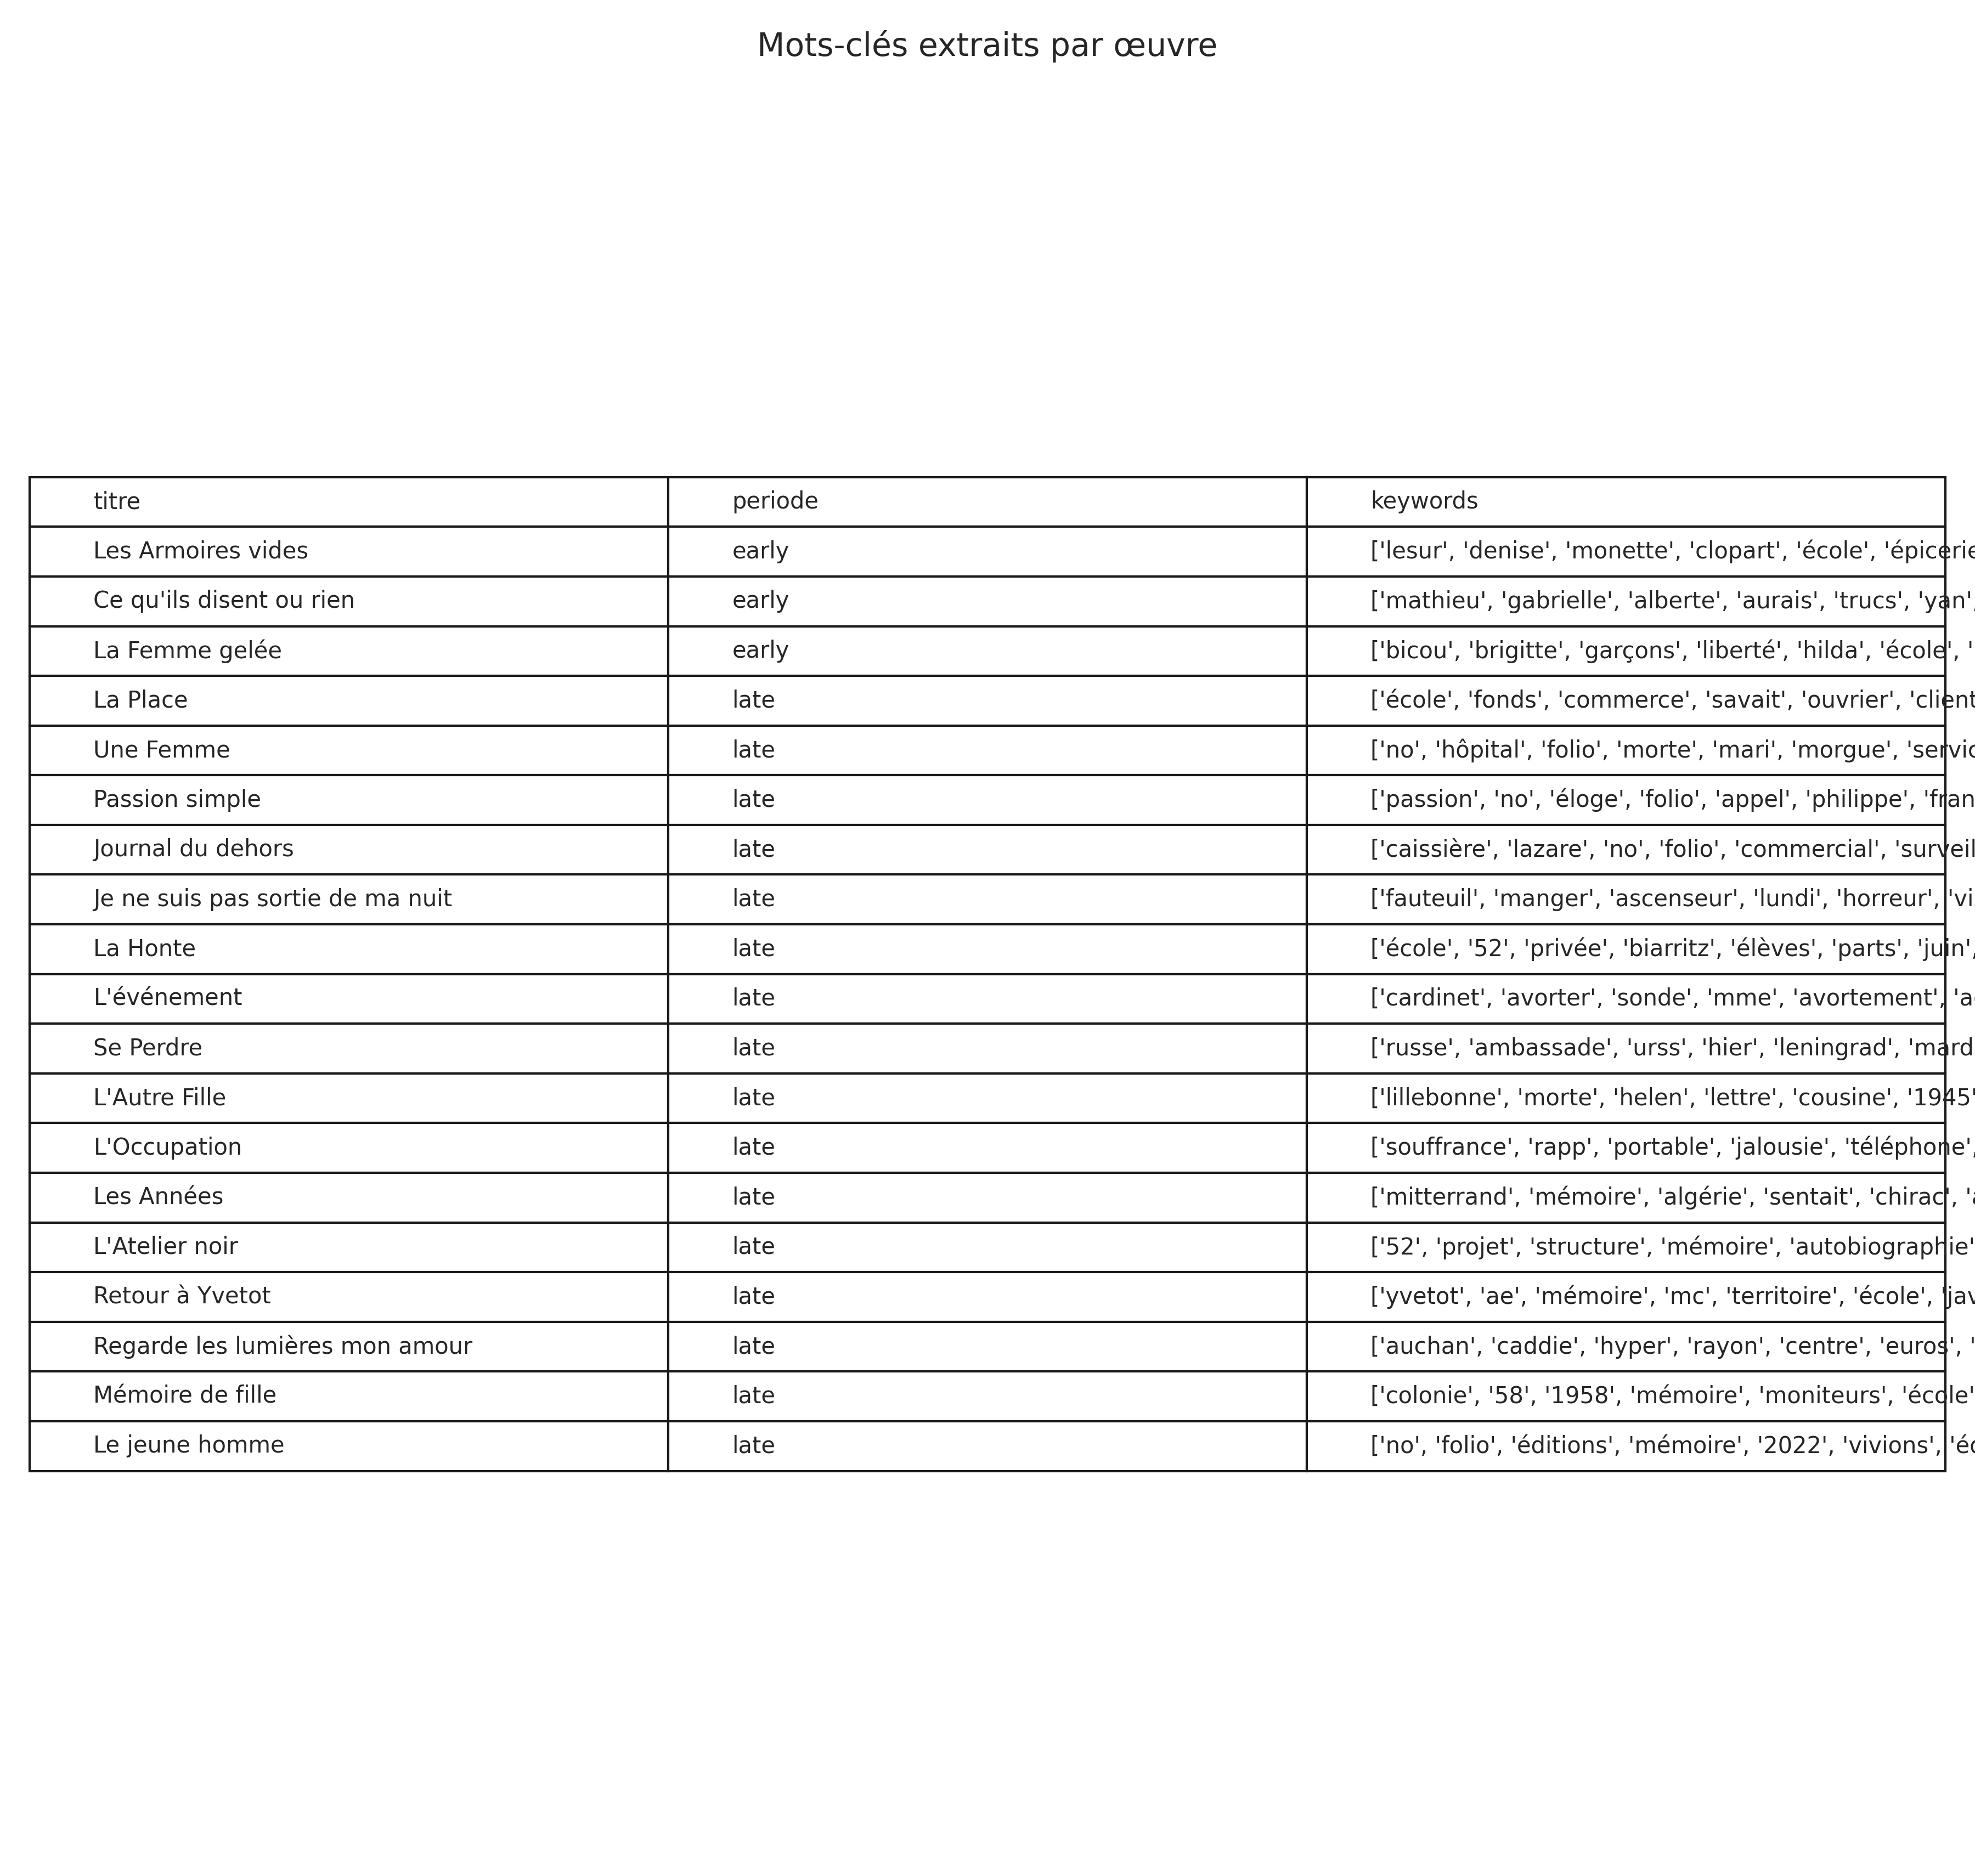
\includegraphics[width=\textwidth]{image/Table_keywords_ernaux.png} % Réduit l'image à 50% de la largeur
        \caption{Liste des mots clés}
        \label{fig:Table de mot-clés des ouvrages d'Ernaux}
    \end{minipage}%
    \hfill
    % Deuxième image à droite
    \begin{minipage}{0.5\textwidth}
        \centering
        \includegraphics[width=\textwidth]{image/Nuages_de_mots_ernaux.png}  % Réduit l'image à 50% de la largeur
        \caption{Nuage de mots}
        \label{fig:Nuage de mots}
    \end{minipage}
\end{figure}

Concernant la classification des thèmes des œuvres, il apparaît que les écrits d'Ernaux se divisent en quatre groupes distincts. Le groupe 0 comprend \textit{Ce qu’ils disent ou rien}, \textit{Je ne suis pas sortie de ma nuit}, \textit{Se Perdre}, \textit{L’Autre Fille}, \textit{L’Occupation} et \textit{Regarde les lumières mon amour}, ces œuvres étant centrées sur des états psychologiques, la solitude, la perte, l’observation et des expériences sociales marginales. Elles présentent une introspection évidente et une écriture spatialement orientée, abordant les frontières sociales telles que la mémoire, l’identité et l’espace urbain. Le groupe 1 inclut \textit{Une Femme}, \textit{Passion simple}, \textit{Journal du dehors}, \textit{L’Événement}, \textit{Les Années}, \textit{L’Atelier noir} et \textit{Le jeune homme}. Ces écrits examinent les expériences féminines et la politique du corps, abordant des thèmes comme l'avortement, les relations amoureuses, les relations mère-fille, et la mémoire historique. Le groupe 2 comprend \textit{Les Armoires vides}, \textit{La Femme gelée}, \textit{La Place} et \textit{La Honte}, où les thèmes se concentrent sur les origines sociales, la mémoire familiale d'enfance et la répression éducative. Le groupe 3 comprend \textit{Retour à Yvetot} et \textit{Mémoire de fille}, qui examinent l'identité régionale, les souvenirs de l’adolescence et le processus de recherche de soi. À travers cette classification, on peut constater que les œuvres d'Ernaux, initialement axées sur des préoccupations familiales et de classe, s’orientent progressivement vers une écriture de mémoire socialisée et historisée, mettant en évidence une évolution profonde de ses thèmes et de son expression personnelle.\\
\begin{figure}[ht!]
    \centering
    \includegraphics[width=\textwidth]{image/Clustering des thèmes de mots-clés de chaque œuvre d'Ernaux.png}
    \caption{Catégorisation thématique}
    \label{fig:Catégorisation thematique}
\end{figure}

 

En ce qui concerne la répartition des temps verbaux, les œuvres d'Ernaux présentent des caractéristiques temporelles distinctes. Le présent de l'indicatif (Indicatif Présent Simple) domine à la fois dans les premiers et derniers travaux, et surtout dans les œuvres récentes, le présent étant davantage utilisé, ce qui correspond à son style d'"autobiographie immédiate" (autobiographie au présent) et renforce le sentiment de présence dans ses écrits. Le passé simple (Passé Simple) est fréquemment employé dans les premières œuvres, utilisé pour les récits linéaires du passé, mais il est progressivement remplacé par le passé composé (Passé Composé) dans les œuvres plus récentes. Le subjonctif présent (Subjonctif Présent Simple) et le conditionnel présent (Conditionnel Présent Simple) sont davantage présents dans les œuvres récentes, notamment dans les explorations des possibilités historiques et des vérités de la mémoire, ce qui témoigne de la réflexion et du doute croissants dans ses écrits. Le présent de l’impératif est pratiquement absent, ce qui reflète le caractère non-directif de son écriture autobiographique.\\
 Répartition des temps verbaux
\begin{figure}[ht!]
    \centering
    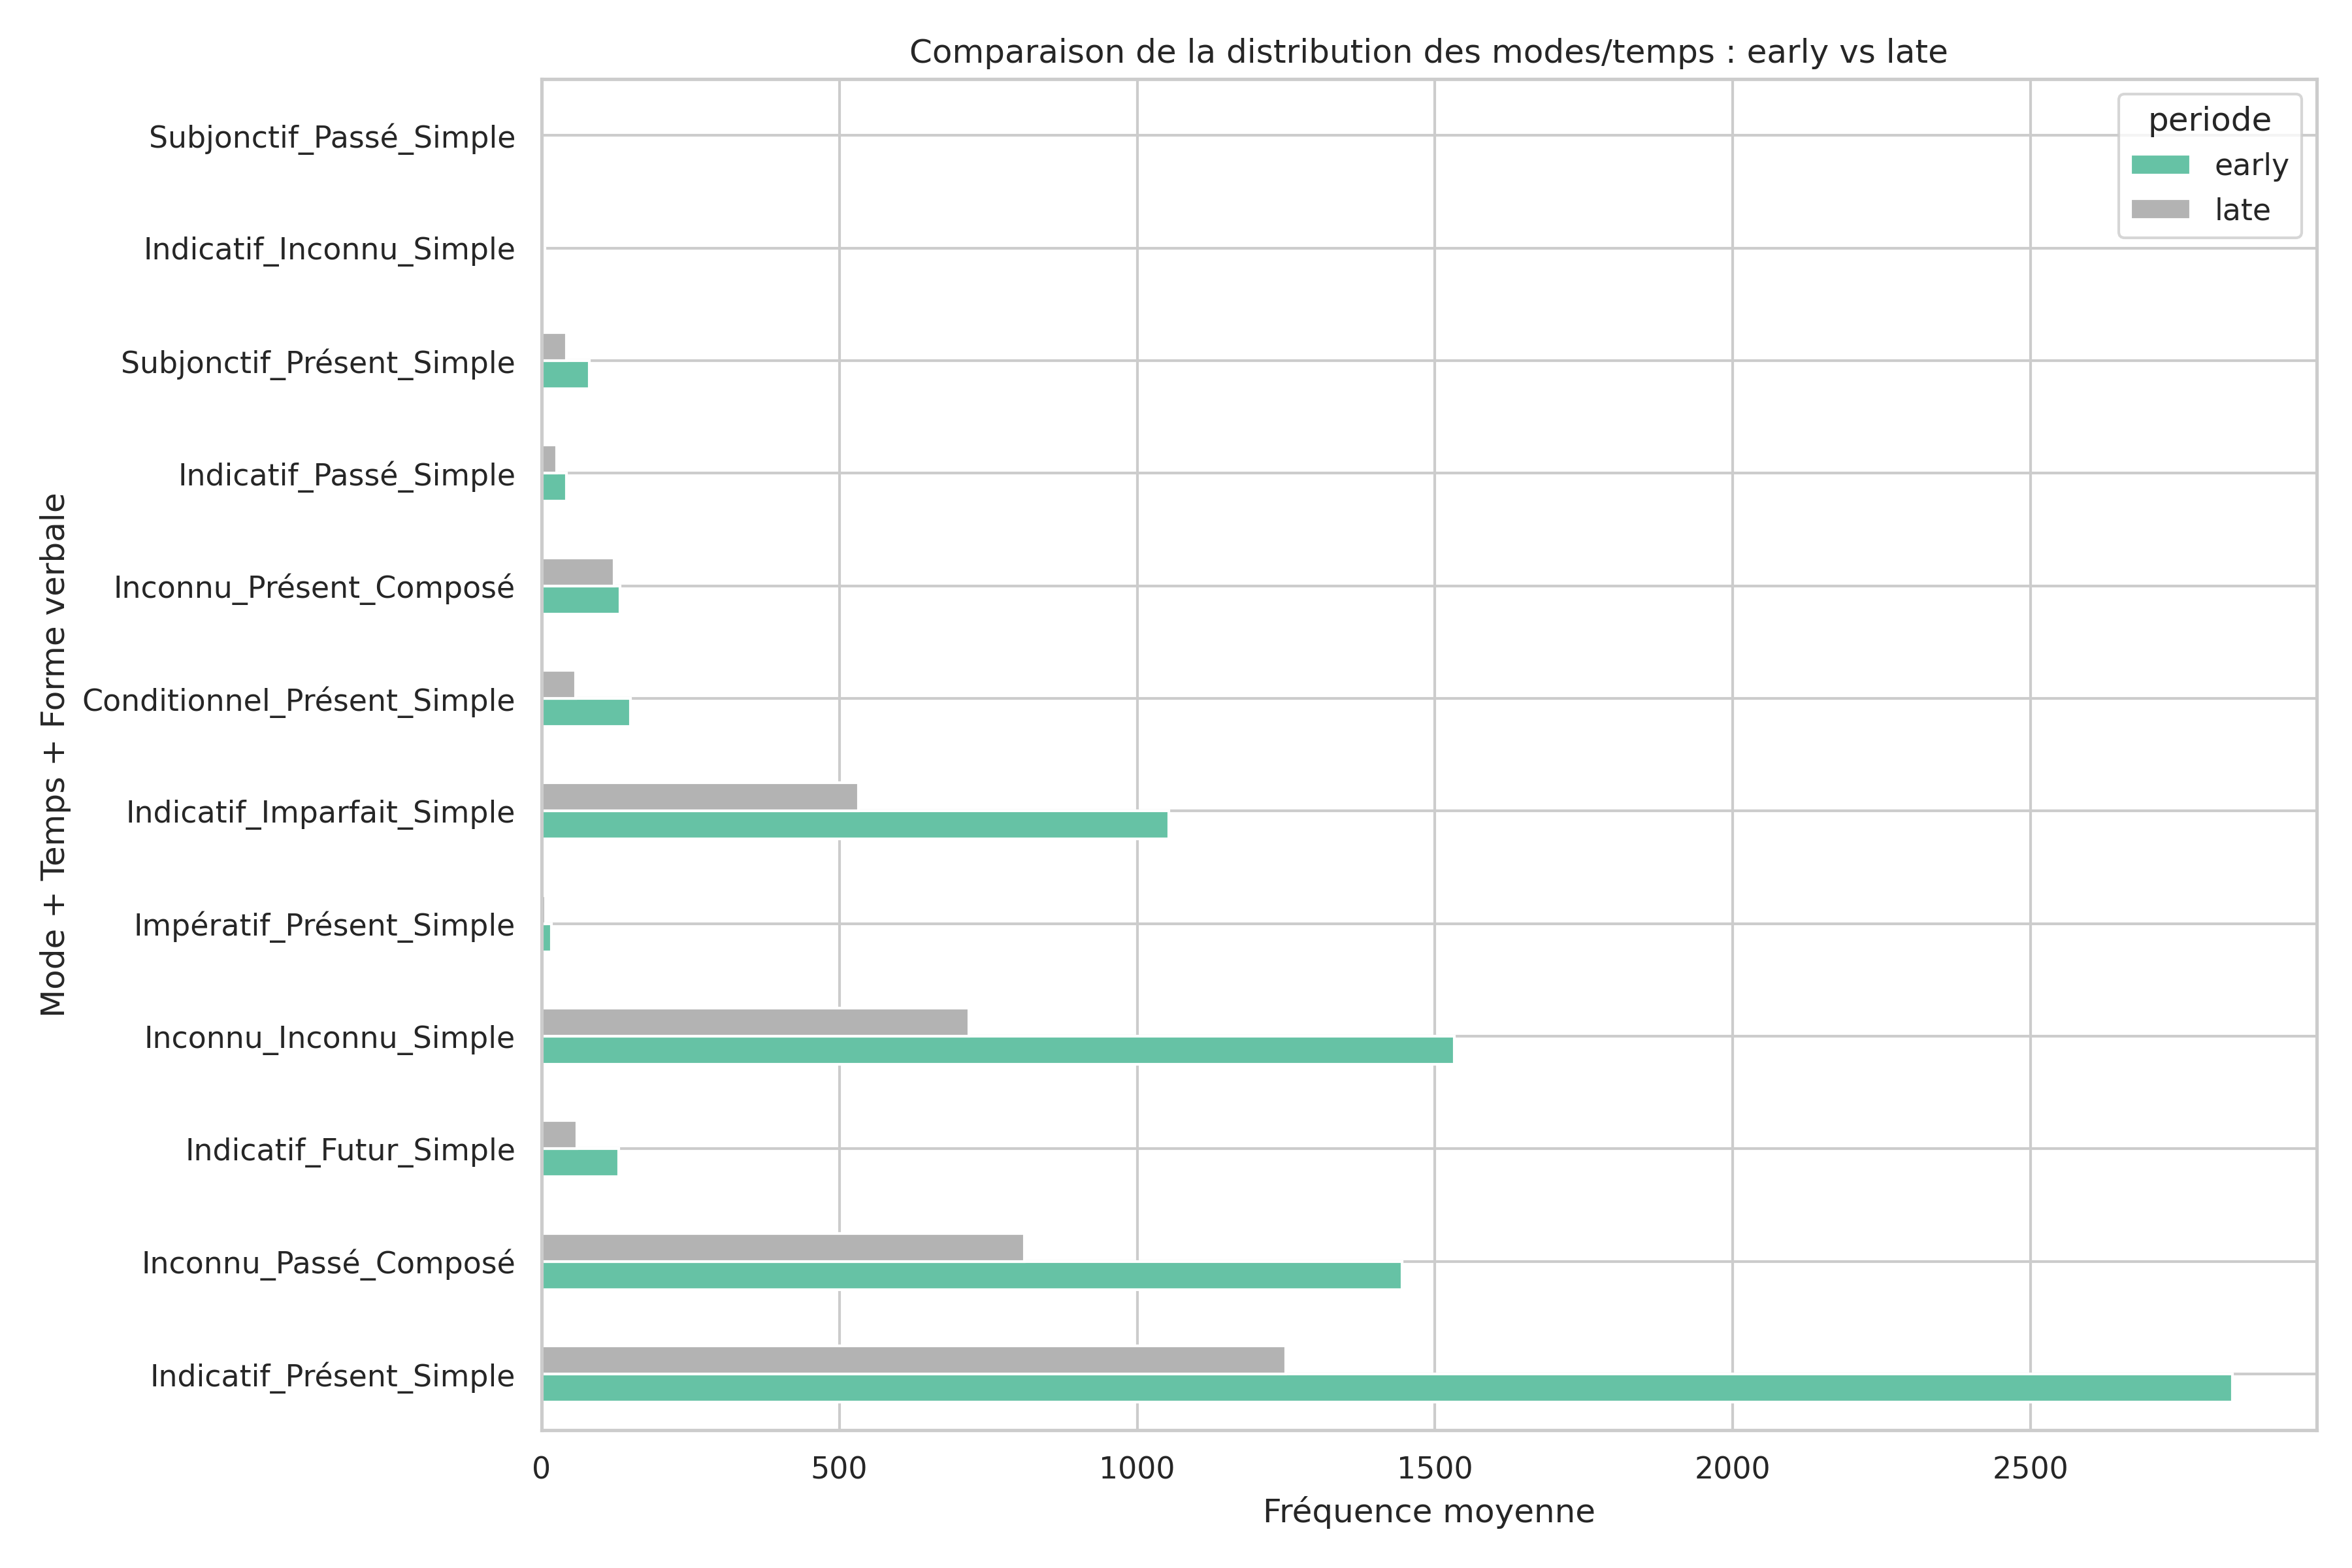
\includegraphics[width=\textwidth]{image/Comparaison_de_la_distribution_des_modes_temps_early_vs_late.png}
    \caption{Répartition des temps verbaux}
    \label{fig:temps verbaux}
\end{figure}

La distribution des pronoms reflète également l’évolution stylistique de l’œuvre d'Ernaux. Le pronom de la première personne "je" domine dans toutes ses œuvres, tant dans les premiers que dans les derniers écrits, avec une légère augmentation dans les œuvres récentes, indiquant un approfondissement de son introspection. Les pronoms de la troisième personne "il" et "elle" deviennent plus fréquents dans ses œuvres tardives, ce qui suggère qu’elle commence à davantage décrire autrui et à réfléchir sur les relations avec les proches ou les "autres" dans la société. L’utilisation du pronom collectif "nous" augmente également dans les œuvres récentes, notamment dans \textit{Les Années}, ce qui illustre l’écriture de la mémoire collective et de l'expérience sociale partagée. Globalement, ses écrits plus tardifs accordent une plus grande attention aux expériences collectives, à la mémoire partagée et aux interactions extérieures, ce qui montre une évolution vers une écriture socialisée et historisée.\\
% Répartition des pronoms
\begin{figure}[ht!]
    \centering
    \includegraphics[width=\textwidth]{image/Fréquence moyenne des pronoms _ early vs late.png}
    \caption{Répartition des pronoms}
    \label{fig:repartition_pronom}
\end{figure}

\newpage

Concernant la distribution du nombre moyen de mots, dans le graphique à barres, nous pouvons observer que certaines œuvres ``récentes'' ont une moyenne de mots par phrase supérieure à celle des œuvres plus anciennes. Par exemple, les phrases dans des œuvres comme \textit{Les Années}, \textit{Ce qu'ils disent ou rien} et \textit{Retour à Yvetot} sont plus longues, ce qui reflète une plus grande complexité. En revanche, certaines œuvres récentes, comme \textit{Passion simple} et \textit{Je ne suis pas sortie de ma nuit}, ont des phrases plus courtes, mettant en avant un style d'écriture plus concis et direct. De manière générale, les œuvres récentes montrent une tendance à la ``diversification'' : certaines adoptent un style minimaliste, tandis que d'autres utilisent des phrases plus longues. Cela indique que la structure des phrases dans les œuvres récentes est devenue plus flexible et variée, reflétant ainsi la diversité du style d'écriture de l'auteure. \\

Dans le diagramme en boîte, nous pouvons observer que les œuvres anciennes (boîte verte) ont une longueur de phrase relativement stable, avec des variations faibles, et une longueur de phrase comprise entre 16 et 25 mots. Cela montre une certaine stabilité et cohérence. En revanche, les œuvres récentes (boîte orange) montrent une plus grande variation, avec des longueurs de phrase allant de 10 à près de 25 mots, indiquant davantage de fluctuation et d'incertitude. Cependant, la plupart des phrases dans les œuvres récentes ont un nombre moyen de mots inférieur à 20, et surtout, dans \textit{Passion simple}, un point bas est observable avec une moyenne de seulement 10,53 mots. La médiane des œuvres récentes est inférieure à celle des œuvres anciennes, ce qui suggère que l'auteure tend à utiliser des phrases plus courtes, probablement pour accentuer la simplicité et la directivité de son langage. Toutefois, la plus grande variation dans les œuvres récentes montre également une complexité accrue du style, témoignant d'une utilisation plus libre et plus diversifiée des structures de phrases.\\
\begin{figure}[ht!]
    \centering
    \begin{subfigure}[b]{0.8\textwidth}
        \centering
        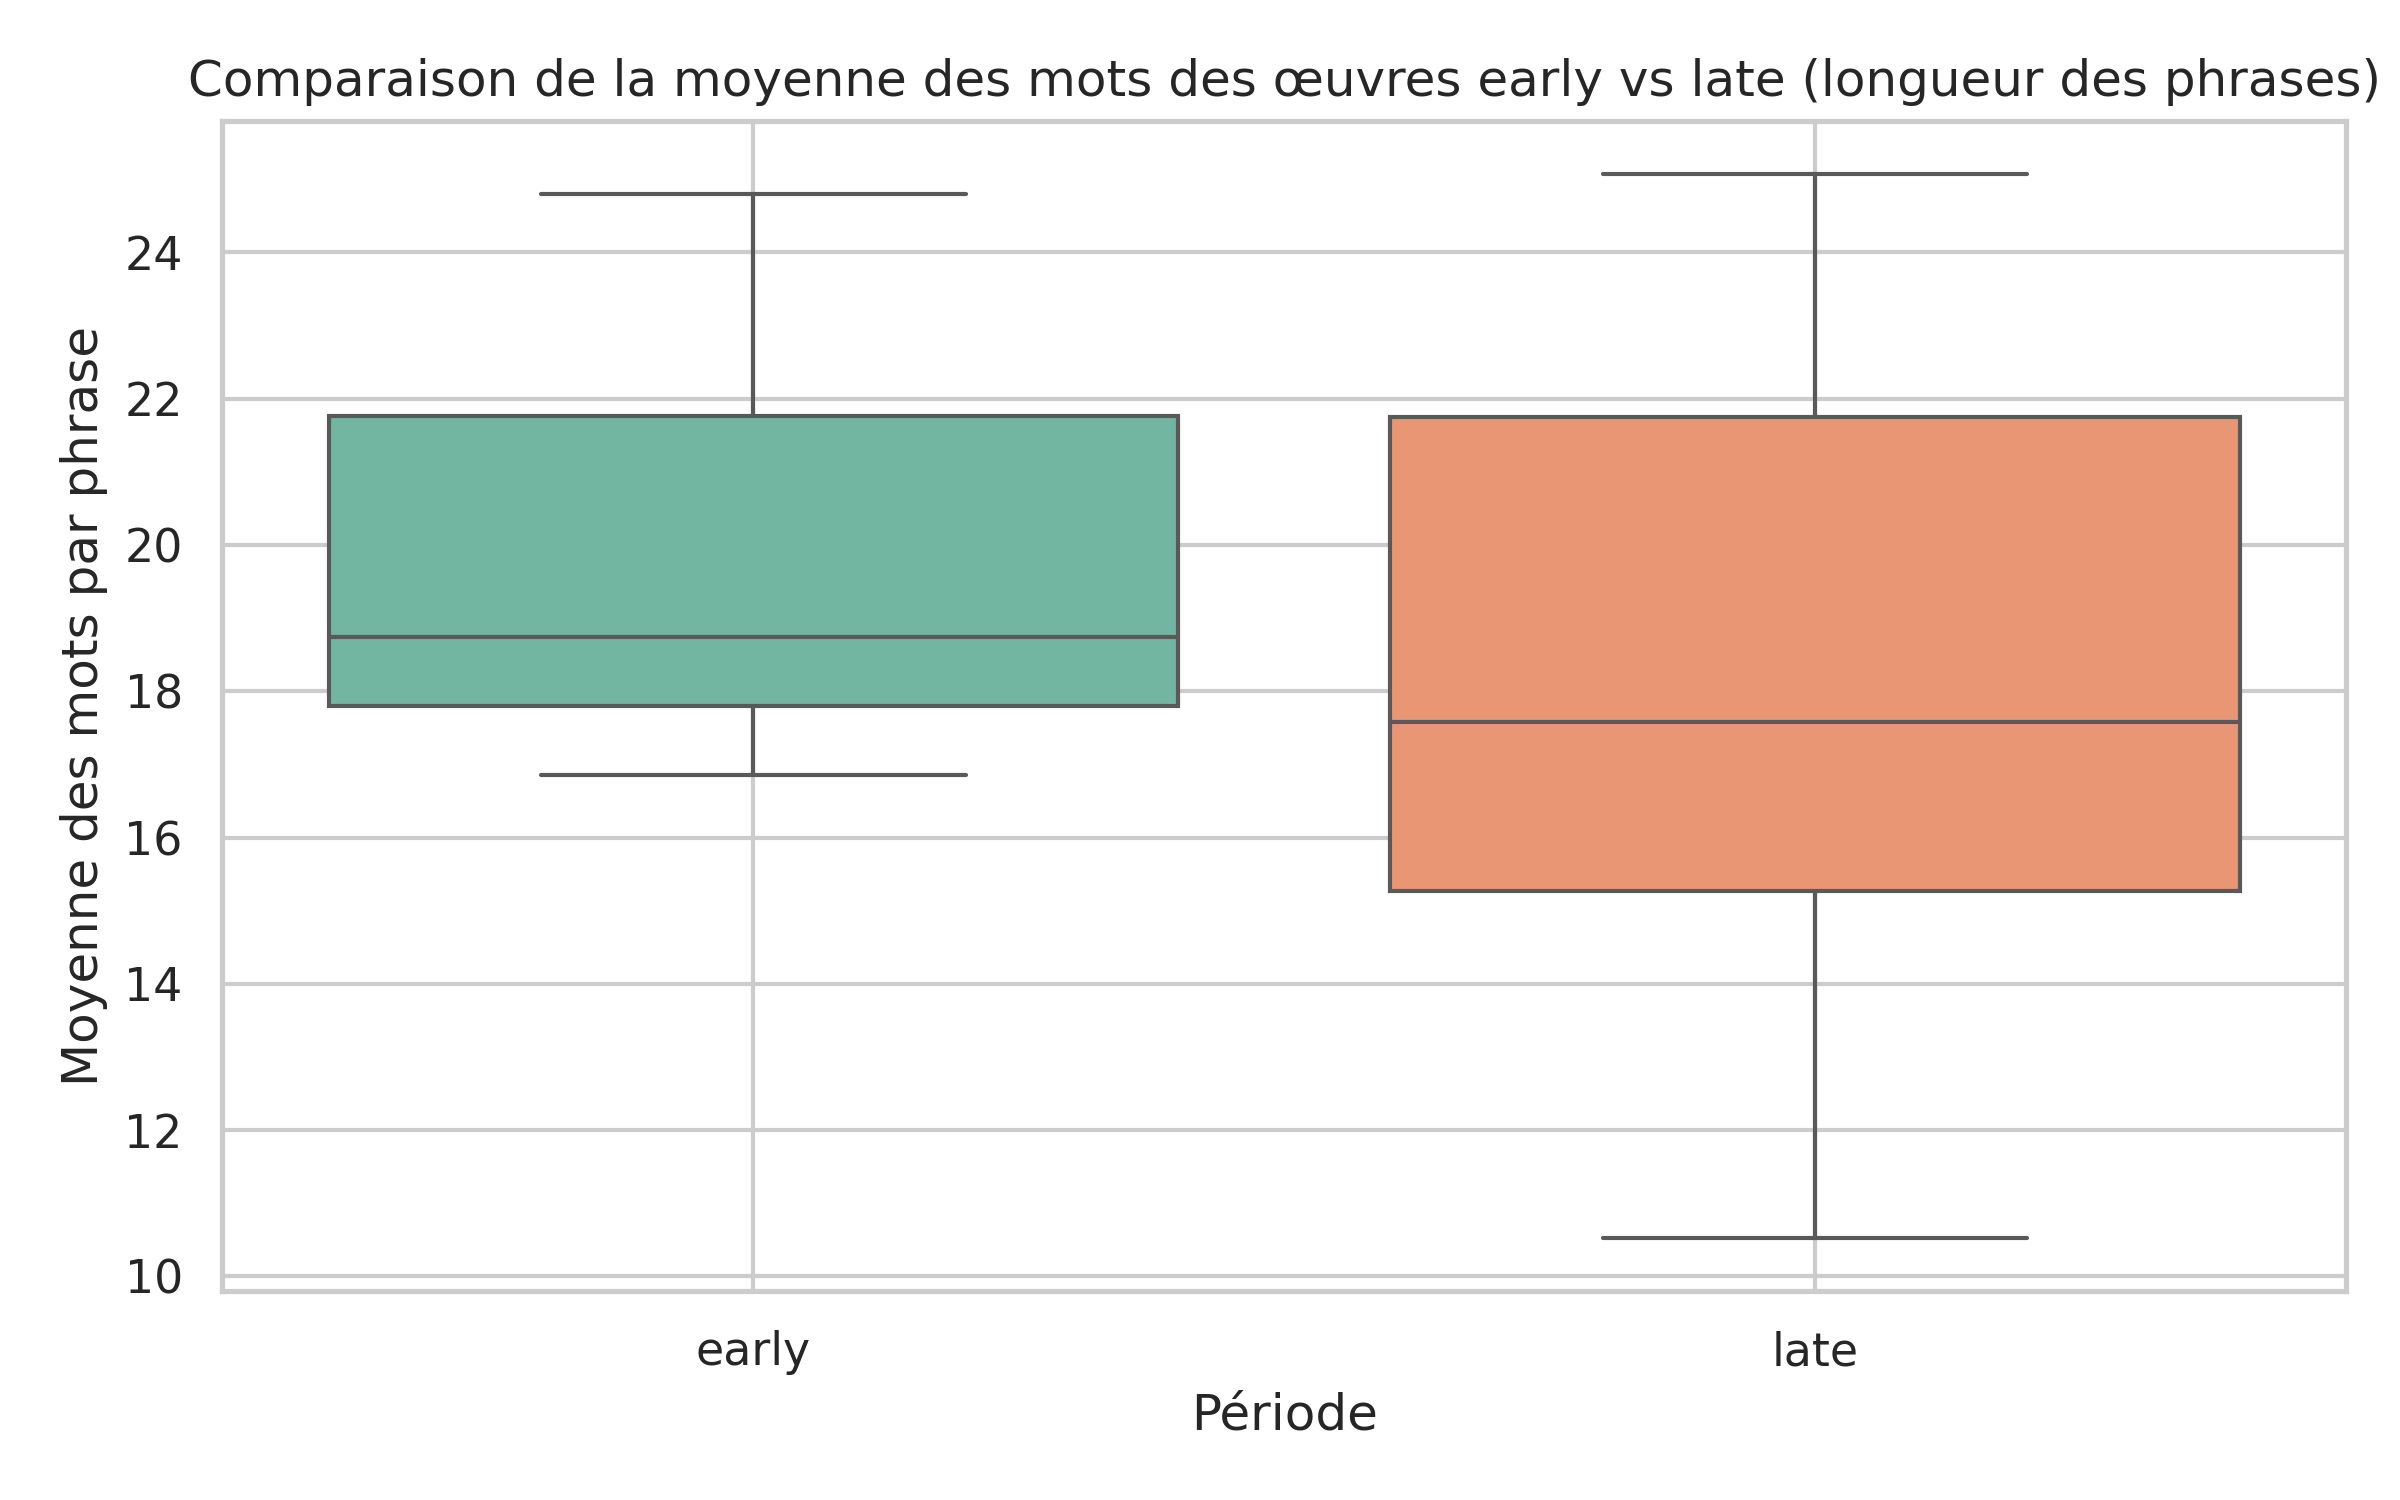
\includegraphics[width=\textwidth]{image/Comparaison de la moyenne des mots des galactiches early vs late (longueur des phrases).png}
        \caption{Répartition des mots moyens (graphique 1)}
        \label{fig:mots_moyens_boite}
    \end{subfigure}
    \vspace{1em} % Espace entre les deux images
    \begin{subfigure}[b]{0.8\textwidth}
        \centering
        \includegraphics[width=\textwidth]{image/Longueur moyenne des phrases de chaque œuvre (par nombre de mots).png}
        \caption{Répartition des mots moyens (graphique 2)}
        \label{fig:mots_moyens_barres}
    \end{subfigure}
    \caption{Comparaison des répartitions des mots moyens entre les œuvres}
    \label{fig:mots_moyens_comparison}
\end{figure}
\newpage
Concernant le TTR (Type-Token Ratio), dans la comparaison des diagrammes en boîte du TTR, la médiane du TTR des œuvres tardives est d'environ 0,48, bien plus élevée que celle des œuvres précoces (environ 0,36). Cette différence indique que les œuvres tardives présentent une plus grande diversité et richesse lexicale. La valeur maximale du TTR des œuvres tardives dépasse largement celle des œuvres précoces, et on observe une plus grande variabilité des textes, ce qui montre que l'auteur adopte une utilisation lexicale plus diversifiée dans ses créations ultérieures. Toutefois, certaines œuvres tardives, comme \textit{Ce qu'ils disent ou rien}, présentent un TTR relativement faible, ce qui suggère que toutes les œuvres tardives ne montrent pas une expansion lexicale significative. En réalité, les œuvres tardives ne sont pas pauvres en vocabulaire, mais elles adoptent une stratégie linguistique plus personnalisée : certaines œuvres utilisent un vocabulaire minimal, tandis que d'autres exhibent une grande variété lexicale.\\

Dans le diagramme en barres du TTR, nous pouvons observer que l'œuvre ayant le TTR le plus élevé parmi les œuvres tardives est \textit{Le jeune homme}, avec un TTR d'environ 0,69, ce qui démontre une utilisation très variée du vocabulaire. En revanche, les œuvres avec une faible richesse lexicale incluent \textit{Se Perdre}, ainsi que les œuvres précoces comme \textit{Les Armoires vides} et \textit{Ce qu'ils disent ou rien}, qui présentent un taux de répétition lexical élevé et traduisent un style d'écriture plus concis. Il est donc clair que toutes les œuvres tardives ne suivent pas la tendance de "simplification" ou de "minimalisme". En fait, l'auteur choisit parfois délibérément d’utiliser un langage plus succinct et répétitif, créant ainsi des contextes et des atmosphères différentes. Par conséquent, les œuvres tardives révèlent une multiplicité de possibilités en termes d’utilisation du vocabulaire : parfois un style minimaliste, parfois une grande fréquence de variation lexicale, ce qui reflète l’exploration plus flexible et diversifiée du langage par l’auteure. En somme, les œuvres précoces et tardives montrent des différences notables dans l'utilisation du vocabulaire et la longueur des phrases, les œuvres tardives présentant un style d’écriture plus riche et diversifié, tout en manifestant une utilisation linguistique plus individualisée, qui reflète différentes stratégies et formes d’expression linguistique.

% Répartition du TTR
\begin{figure}[ht!]
    \centering
    \includegraphics[width=\textwidth]{image/Comparaison de la richesse lexicale des œuvres early et late (TTR).png}
    \caption{Répartition du TTR}
    \label{fig:repartition_TTR_boite}
\end{figure} 
\begin{figure}[ht!]
    \centering
    \includegraphics[width=\textwidth]{image/Répartition de la richesse lexicale des œuvres (TTR).png}
    \caption{Répartition du TTR}
    \label{fig:repartition_TTR_barres}
\end{figure} 

\newpage

\subsection{Analyse syntaxique}
Les structures des phrases dans les premiers et derniers travaux d'Ernaux diffèrent de manière marquée. Dans les premières œuvres, la longueur moyenne des phrases reste relativement stable, généralement entre 16 et 25 mots, tandis que dans les œuvres récentes, la longueur des phrases varie davantage, surtout dans \textit{Passion simple} et \textit{Je ne suis pas sortie de ma nuit}, où l’on observe des phrases plus courtes. Les œuvres récentes tendent vers une syntaxe plus concise, bien qu’il y ait également des phrases plus longues, reflétant une diversification de son style. De plus, la richesse lexicale (TTR) augmente de manière significative dans les œuvres récentes, ce qui témoigne d’une utilisation plus variée du vocabulaire. Bien que certaines œuvres récentes comme \textit{Ce qu’ils disent ou rien} présentent un TTR plus bas, elles présentent globalement une stratégie linguistique plus individualisée.\\
% Catégories grammaticales 
\begin{figure}[ht!]
    \centering
    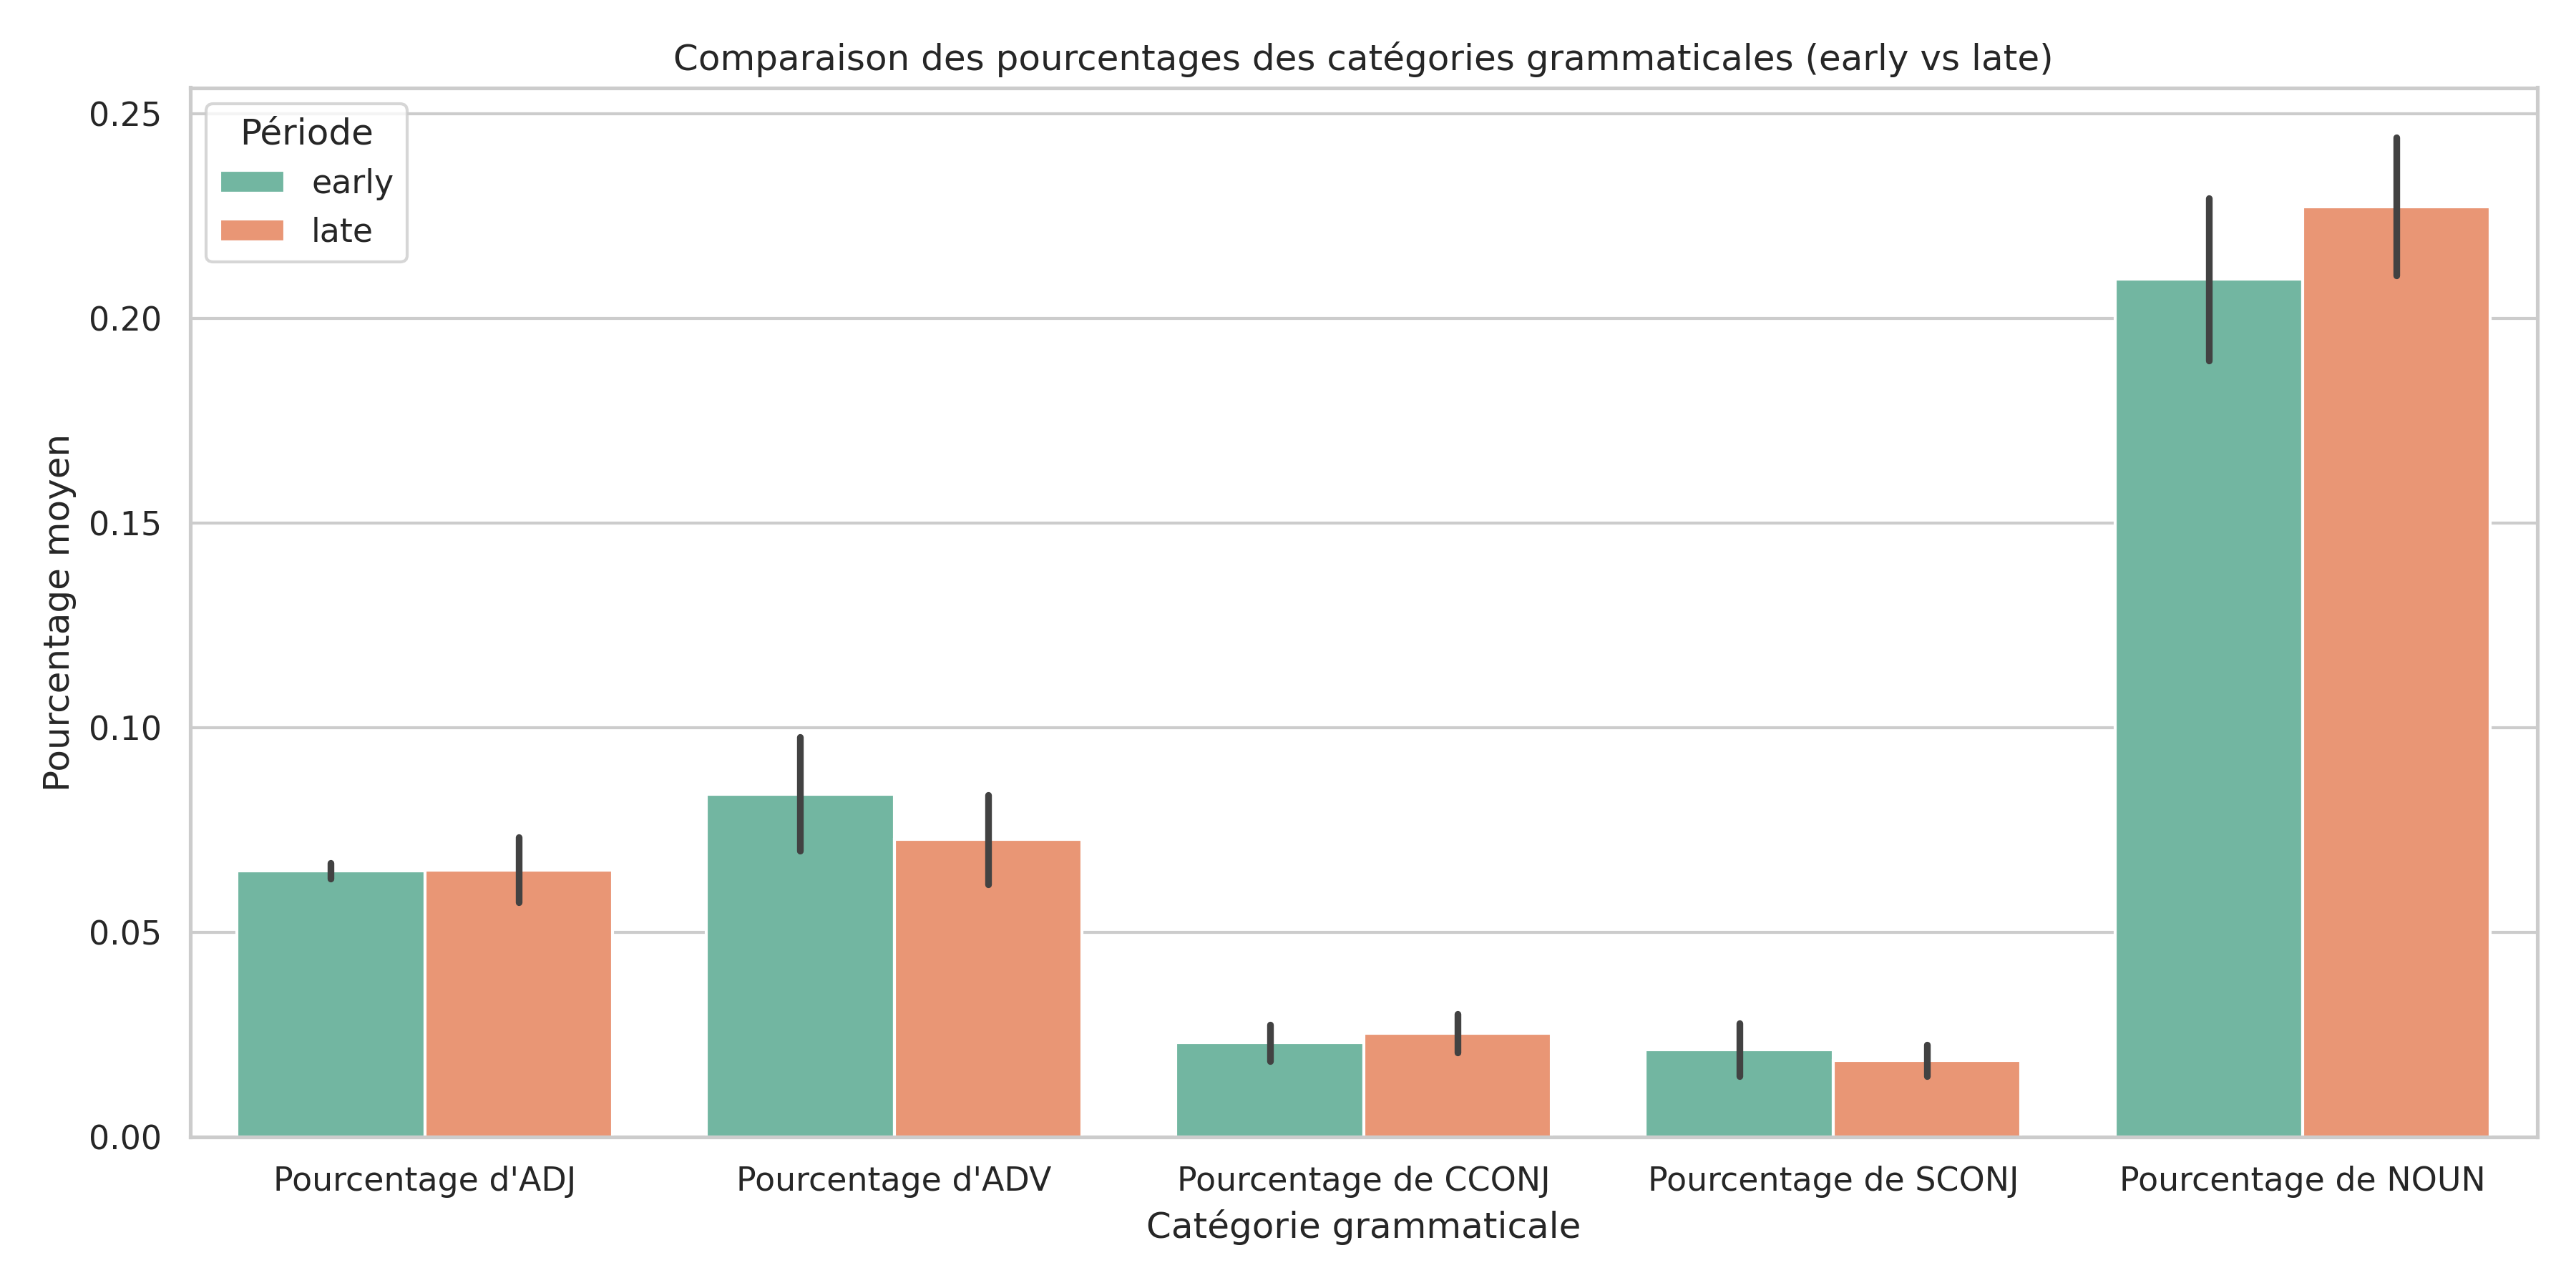
\includegraphics[width=\textwidth]{image/Comparaison des pourcentages des catégories grammaticales (early vs late).png}
    \caption{Répartition des catégories grammaticales}
    \label{fig:catégories grammaticales}
\end{figure}

\newpage

\subsection{Analyse rhétorique}
Les œuvres d'Ernaux présentent une utilisation relativement sobre de la répétition. La plupart de ses textes montrent une faible densité de répétition, en particulier dans les œuvres non-diatétiques. Cependant, dans \textit{Je ne suis pas sortie de ma nuit}, en raison de son format de journal, la répétition est plus présente et contribue à une intensification expressive. L'utilisation des parallélismes est assez rare et se retrouve principalement dans les œuvres plus récentes comme \textit{Une femme} et \textit{Passion simple}, où les structures parallèles et les phrases structurées renforcent le rythme et l’intensité de l’écriture.\\

D'après ces analyses, les indicateurs quantitatifs du "style simple" sont définis par une moyenne de TTR de 0.4 et une longueur moyenne de phrase de 18 mots. Les œuvres d'Ernaux, avec leurs caractéristiques en termes de TTR et de longueur des phrases, répondent aux critères du style simple, en particulier dans ses premiers écrits où le TTR est plus bas, tandis que les œuvres récentes montrent une réduction de la longueur des phrases, ce qui témoigne d'un style d'écriture plus concis.
% Répartition des répétitions
\begin{figure}[ht!]
    \centering
    \includegraphics[width=\textwidth]{image/Densité de repetition_density par œuvre.png}
    \caption{Répartition des répétitions}
    \label{fig:repartition_repetitions}
\end{figure}

\vspace{1cm}

% Répartition des parallélismes
\begin{figure}[ht!]
    \centering
    \includegraphics[width=\textwidth]{image/Densité de parallelism_density par œuvre.png}
    \caption{Répartition des parallélismes}
    \label{fig:repartition_parallels}
\end{figure}

\newpage

\section{Corpus externe}
Dans le corpus externe, l’analyse du TTR et de la longueur moyenne des phrases d’autres écrivains montre des similitudes et des différences avec le style d'Ernaux. Par exemple, le TTR de Yourcenar varie entre 0.45 et 0.5, avec des phrases généralement plus longues (plus de 20 mots), ce qui reflète un style plus complexe et élégant ; celui de Robbe-Grillet est plus bas (environ 0.35), avec des phrases plus courtes (entre 15 et 18 mots), représentant son style de description précis et minimaliste caractéristique du "nouveau roman" ; le TTR de Sartre est plus élevé (environ 0.5), et ses phrases sont plus longues, ce qui reflète une structure complexe et un texte à forte dimension philosophique ; Simon a un TTR élevé et des phrases relativement courtes, caractérisant un style sobre ; enfin, Pinget et Green présentent un TTR bas avec des phrases courtes, ce qui témoigne d’un style simple et direct.\\

Comparé à ces écrivains, le style d'Ernaux se situe dans le cadre de l’écriture "simple". En effet, le TTR d'Ernaux est relativement bas, et la longueur de ses phrases est courte, ce qui le rapproche du style de Robbe-Grillet. Toutefois, son écriture se distingue par une dimension sociologique et historique plus marquée. Elle utilise un vocabulaire précis pour analyser les classes sociales et décrire des expériences corporelles, ce qui crée une autobiographie distinctive. Parmi les écrivains du corpus externe, le style d'Ernaux se distingue, particulièrement dans l’utilisation du vocabulaire, et même si son TTR est légèrement plus élevé que celui de Robbe-Grillet, il demeure plus simple et direct que celui de Sartre, tout en mettant l’accent sur le contexte social et historique.
\begin{figure}[ht!]
    \centering
    \begin{subfigure}[b]{0.8\textwidth}
        \centering
        \includegraphics[width=\textwidth]{image/TTR par œuvre (corpus externe).png}
        \caption{Répartition du TTR pour chaque œuvre}
        \label{fig:TTR_externe}
    \end{subfigure}
    
    \vspace{0.5cm} % Ajouter un peu d'espace entre les deux images

    \begin{subfigure}[b]{0.8\textwidth}
        \centering
        \includegraphics[width=\textwidth]{image/Longueur moyenne des phrases par œuvre (corpus externe).png}
        \caption{Répartition du nombre moyen de mots pour chaque œuvre}
        \label{fig:mots_moyens_externe}
    \end{subfigure}
\end{figure}


% Conclusion
\chapter{Conclusion et perspectives}
\label{chap:Conclusion_et_perspectives}
Après cette étude, nous pouvons conclure que les œuvres d'Annie Ernaux ne sont pas absolument "binarisées". Bien que nous puissions observer des différences entre ses œuvres précoces et tardives dans certains aspects, tels que la longueur des phrases et la richesse lexicale, ces différences ne sont pas absolues. En effet, certaines œuvres tardives montrent une tendance vers un style plus simple et minimaliste (comme \textit{Passion simple} et \textit{Je ne suis pas sortie de ma nuit}), tandis que d'autres adoptent des phrases plus longues (comme \textit{Les Années} et \textit{Retour à Yvetot}). De plus, bien que les œuvres d'Ernaux présentent des évolutions en termes de syntaxe et de rhétorique, certains éléments restent présents tout au long de ses œuvres. Par exemple, l'utilisation fréquente de la répétition semble être un moyen pour elle de s'explorer elle-même et de revenir sur son passé. Ces évolutions suggèrent que le travail d'Ernaux présente une tendance à la "diversification" plutôt qu'une séparation stricte en deux catégories. Par conséquent, nous pouvons considérer que son changement de style est un processus graduel plutôt qu'une rupture totale.\\

Concernant l’analyse du corpus externe, les œuvres d’Annie Ernaux manifestent généralement une caractéristique de "style réaliste", en particulier dans la description de la vie quotidienne, des émotions personnelles et des contextes sociaux. Elle utilise un langage simple et direct. Cependant, ce "style réaliste" n’est pas propre à Ernaux ; il s'agit d'une caractéristique courante parmi ses contemporains. De nombreux écrivains, en particulier ceux représentant la littérature autobiographique et réaliste, ont tendance à utiliser un langage simple et direct pour décrire des expériences personnelles et des réalités sociales. Par exemple, des auteurs tels qu'Albert Camus ou Michel Houellebecq utilisent également un style d'écriture épuré. Toutefois, le "style réaliste" d'Ernaux se distingue par sa finesse émotionnelle et son observation unique des changements sociaux, ce qui lui confère une dimension personnelle et distinctive.\\

Quant aux limites de cette recherche, il convient de noter que l’analyse du vocabulaire et de la structure syntaxique n’a pas été assez approfondie. En effet, la structure des phrases est extrêmement complexe, car elle dépend non seulement de la combinaison des mots, mais aussi des relations et interactions entre les différents éléments de la phrase. Dans cette étude, nous nous sommes principalement concentrés sur la longueur moyenne des phrases et certains indicateurs de base concernant les classes grammaticales des mots. Cependant, ces méthodes sont trop simplistes pour rendre compte de la multidimensionnalité de la structure des phrases. Pour mieux comprendre les couches structurelles des phrases et les relations internes entre leurs composants, nous avons besoin d'outils d'analyse syntaxique plus précis. Comme l'exemple donné par Yuanfeng Lu dans \cite{lu2021caracterisation}\textit{Caractérisation des styles littéraires par l'extraction automatique des patrons syntaxiques dans des romans français du 19ème siècle}, l'utilisation d'un arbre syntaxique permet de rendre plus claires les structures et les relations hiérarchiques entre les différents composants de la phrase. Par exemple, dans les phrases complexes, la combinaison des verbes, noms et adjectifs ne suit pas une simple superposition linéaire, mais crée une structure hiérarchique par des règles grammaticales spécifiques, une dimension que nous n'avons pas suffisamment explorée.\\

Enfin, comme l’indique Garric, N. dans \cite{garric2011vers} "Comme il a été souligné, un référentiel conçu sur la base des seuls marqueurs linguistiques serait insuffisant pour l’analyse stylistique notamment déterminée par des interprétants génériques". Dans notre étude, le corpus externe utilisé comprend de nombreux romans, certains avec des caractéristiques autobiographiques, tandis que le corpus interne d'Ernaux est principalement composé de romans autobiographiques, mais aussi de journaux (comme \textit{Journal du dehors} et \textit{Regarde les lumières mon amour}) et de mémoires (comme \textit{Les Années}). Les différences de genre entre ces deux corpus peuvent avoir un impact potentiel sur les résultats de l’analyse.\\


Pour les recherches futures, je souhaiterais explorer davantage les caractéristiques linguistiques du corpus externe, tout en élargissant ce dernier pour étudier en profondeur le style d'écriture des autres auteurs contemporains. Parallèlement, j’espère pouvoir approfondir l’étude des styles d’écriture des écrivaines contemporaines en me basant sur les recherches liées à la longueur des phrases dans leurs œuvres.




%Bibliographie
\bibliographystyle{apalike}
\bibliography{bibliograhie}
 

\end{document}